\begin{figure}[H]
	\centering
		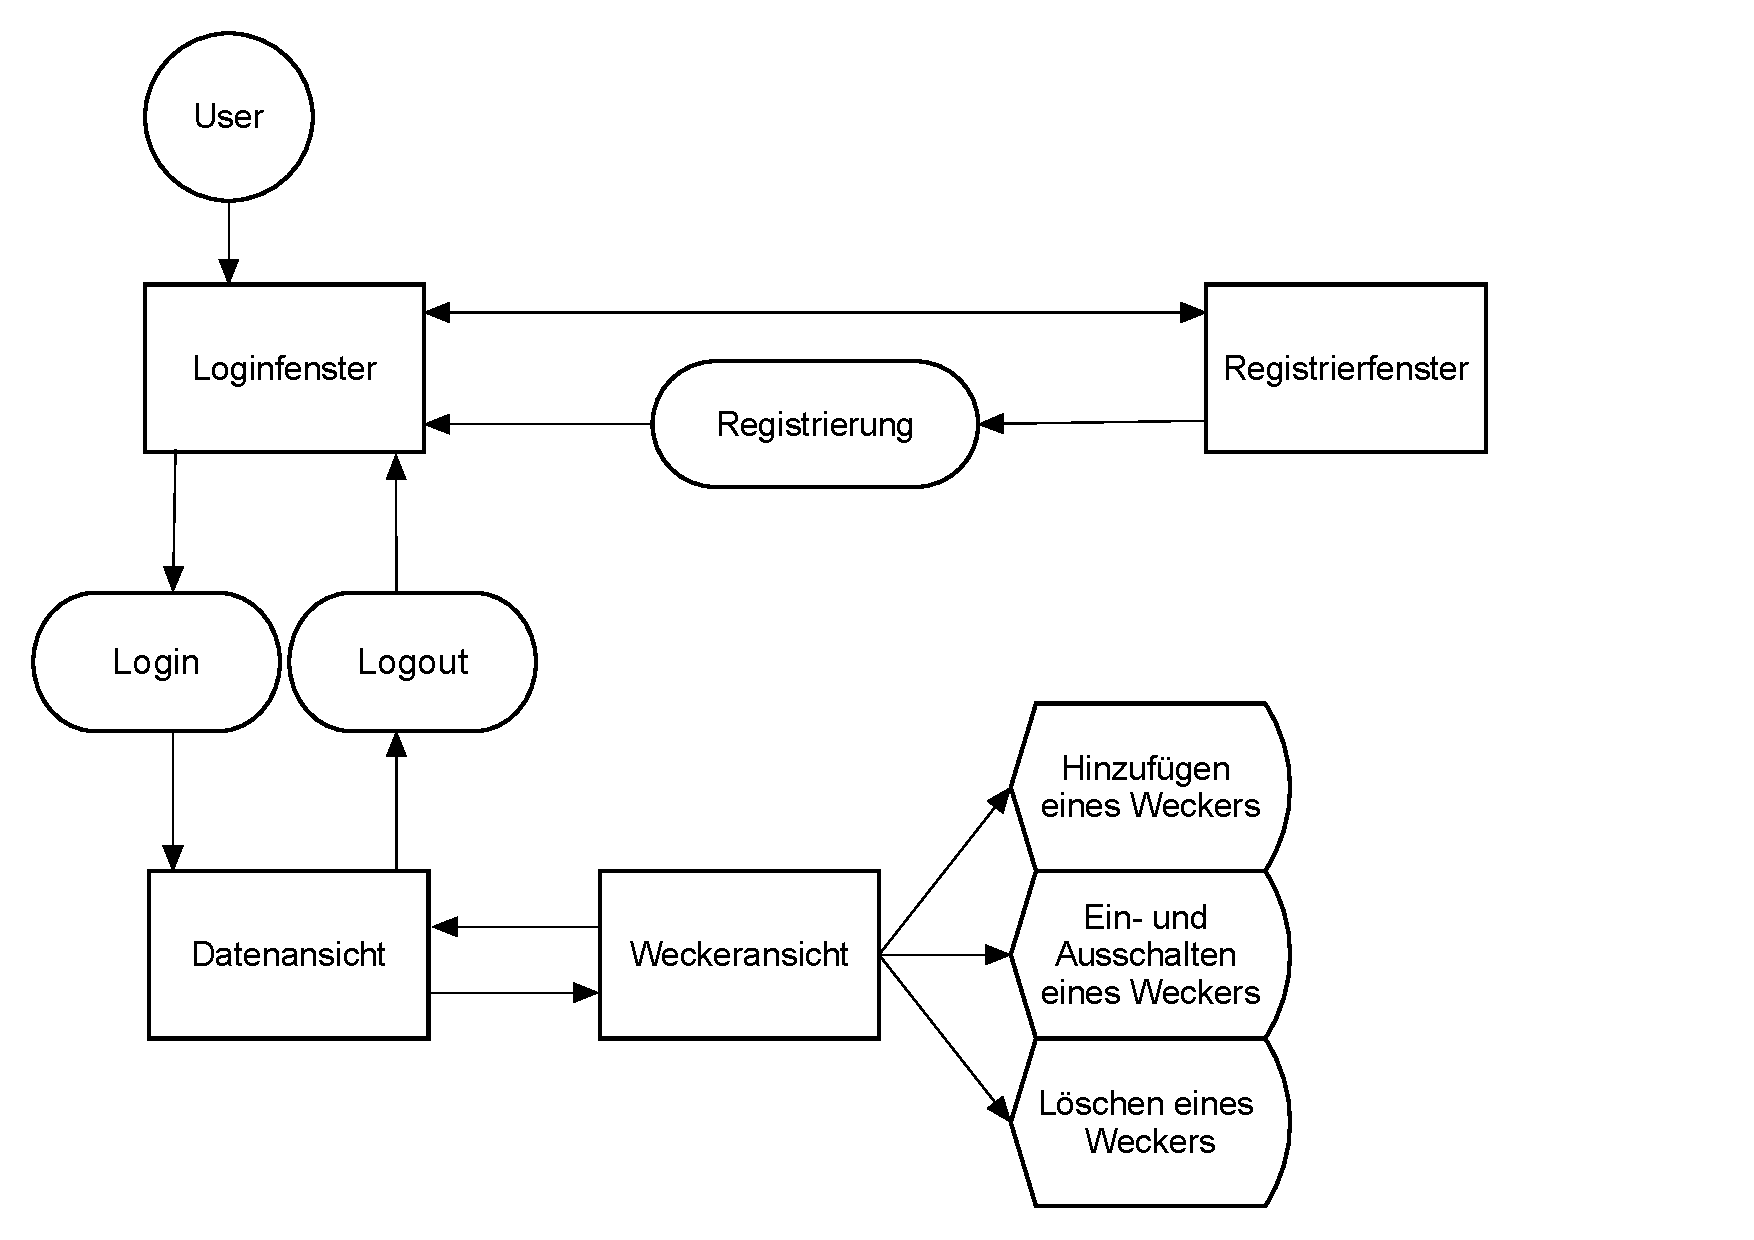
\includegraphics[width=0.9\textwidth]{Gartner/assets/flussdiagramm.pdf}
	\caption{Flussdiagramm der Mobile Application}
	\label{fig:MA_Flussdiagramm}
\end{figure}

\begin{figure}[H]
	\centering
		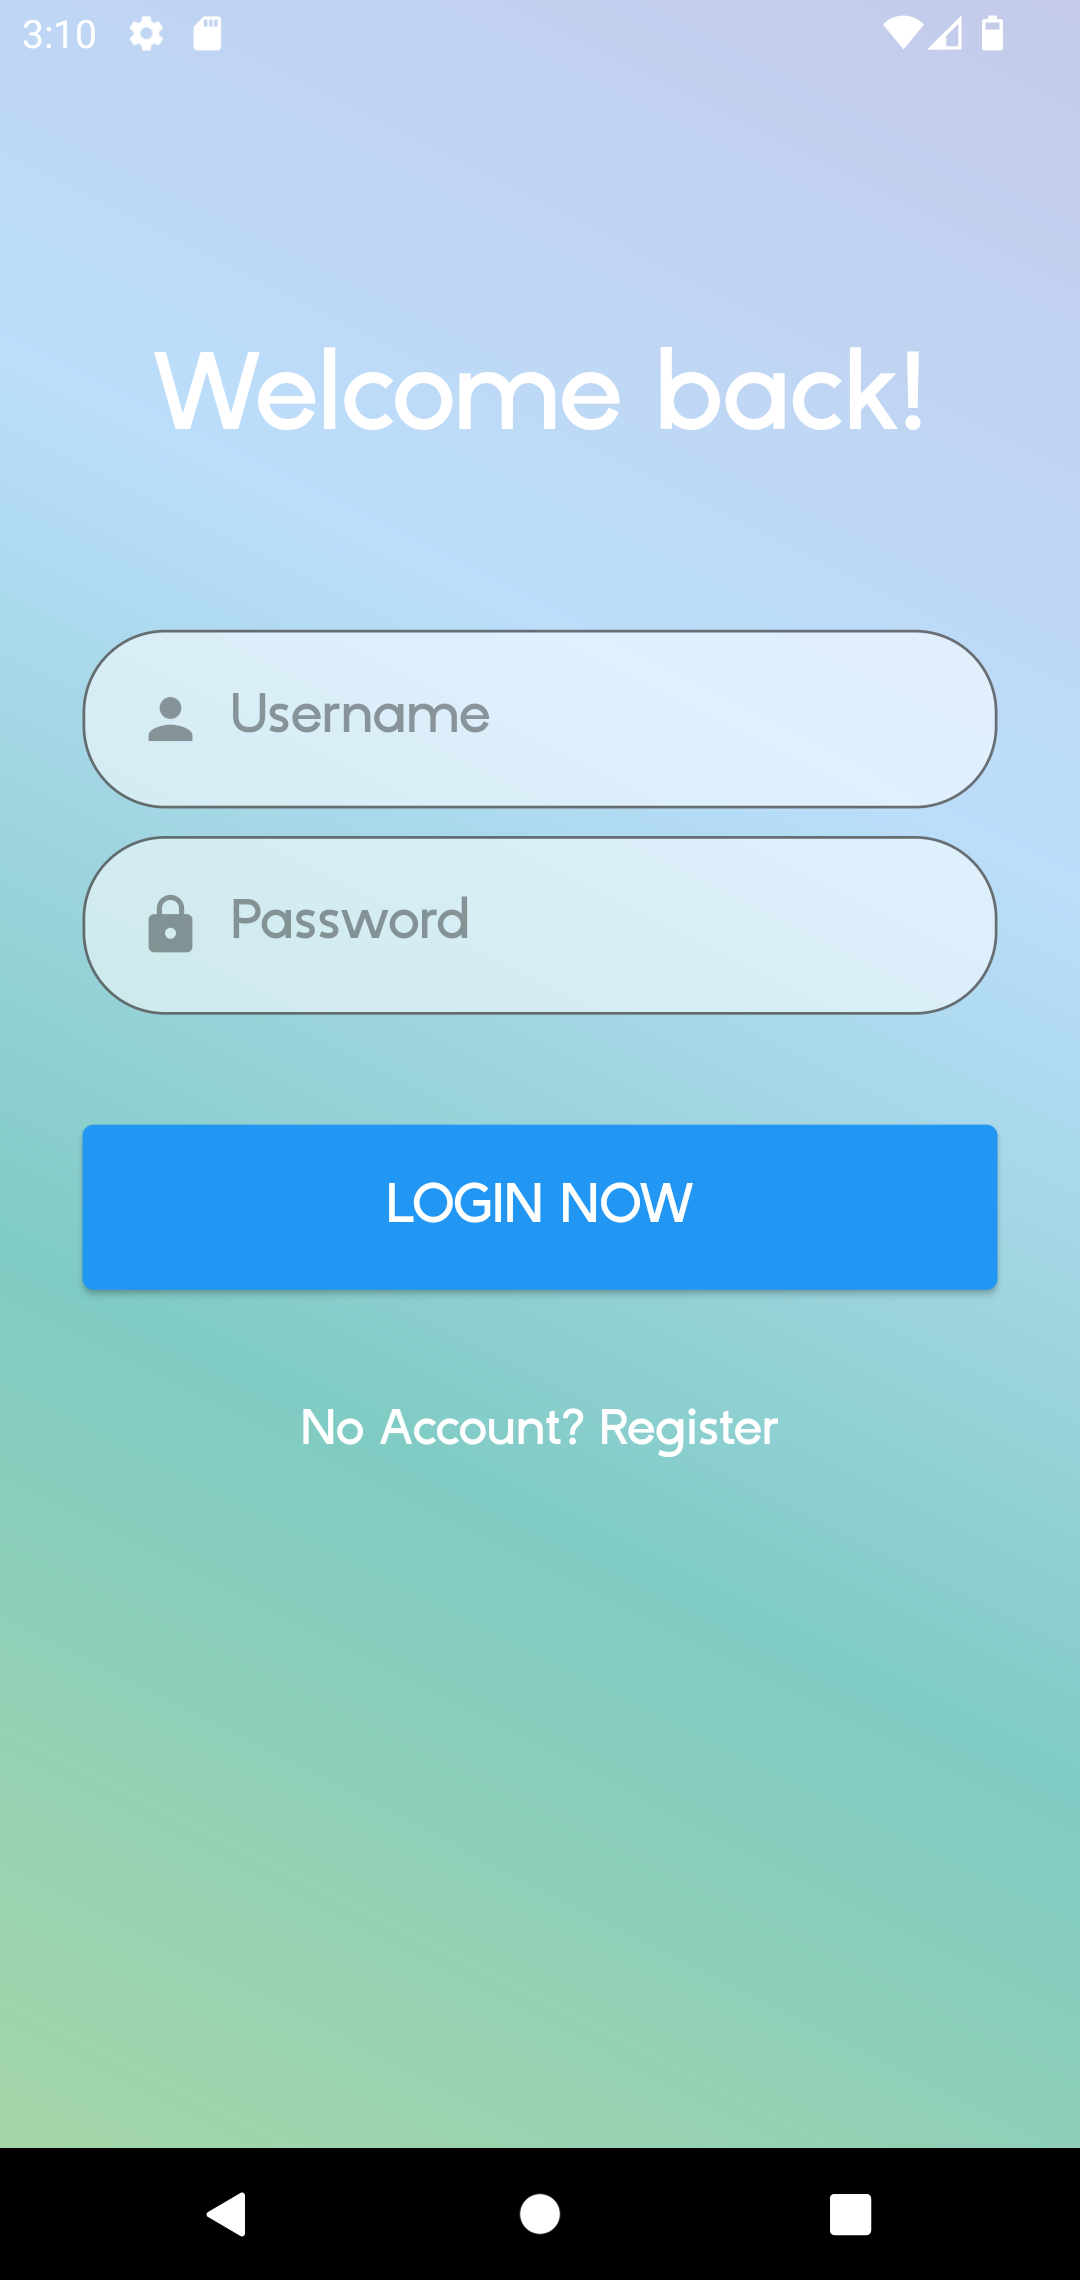
\includegraphics[width=0.3\textwidth]{Gartner/assets/ss_MAFlussdiagramm_loginfenster.png}
	\caption{Loginfenster des GUI}
	\label{fig:MA_Loginfenster}
\end{figure}

\begin{figure}[H]
	\centering
		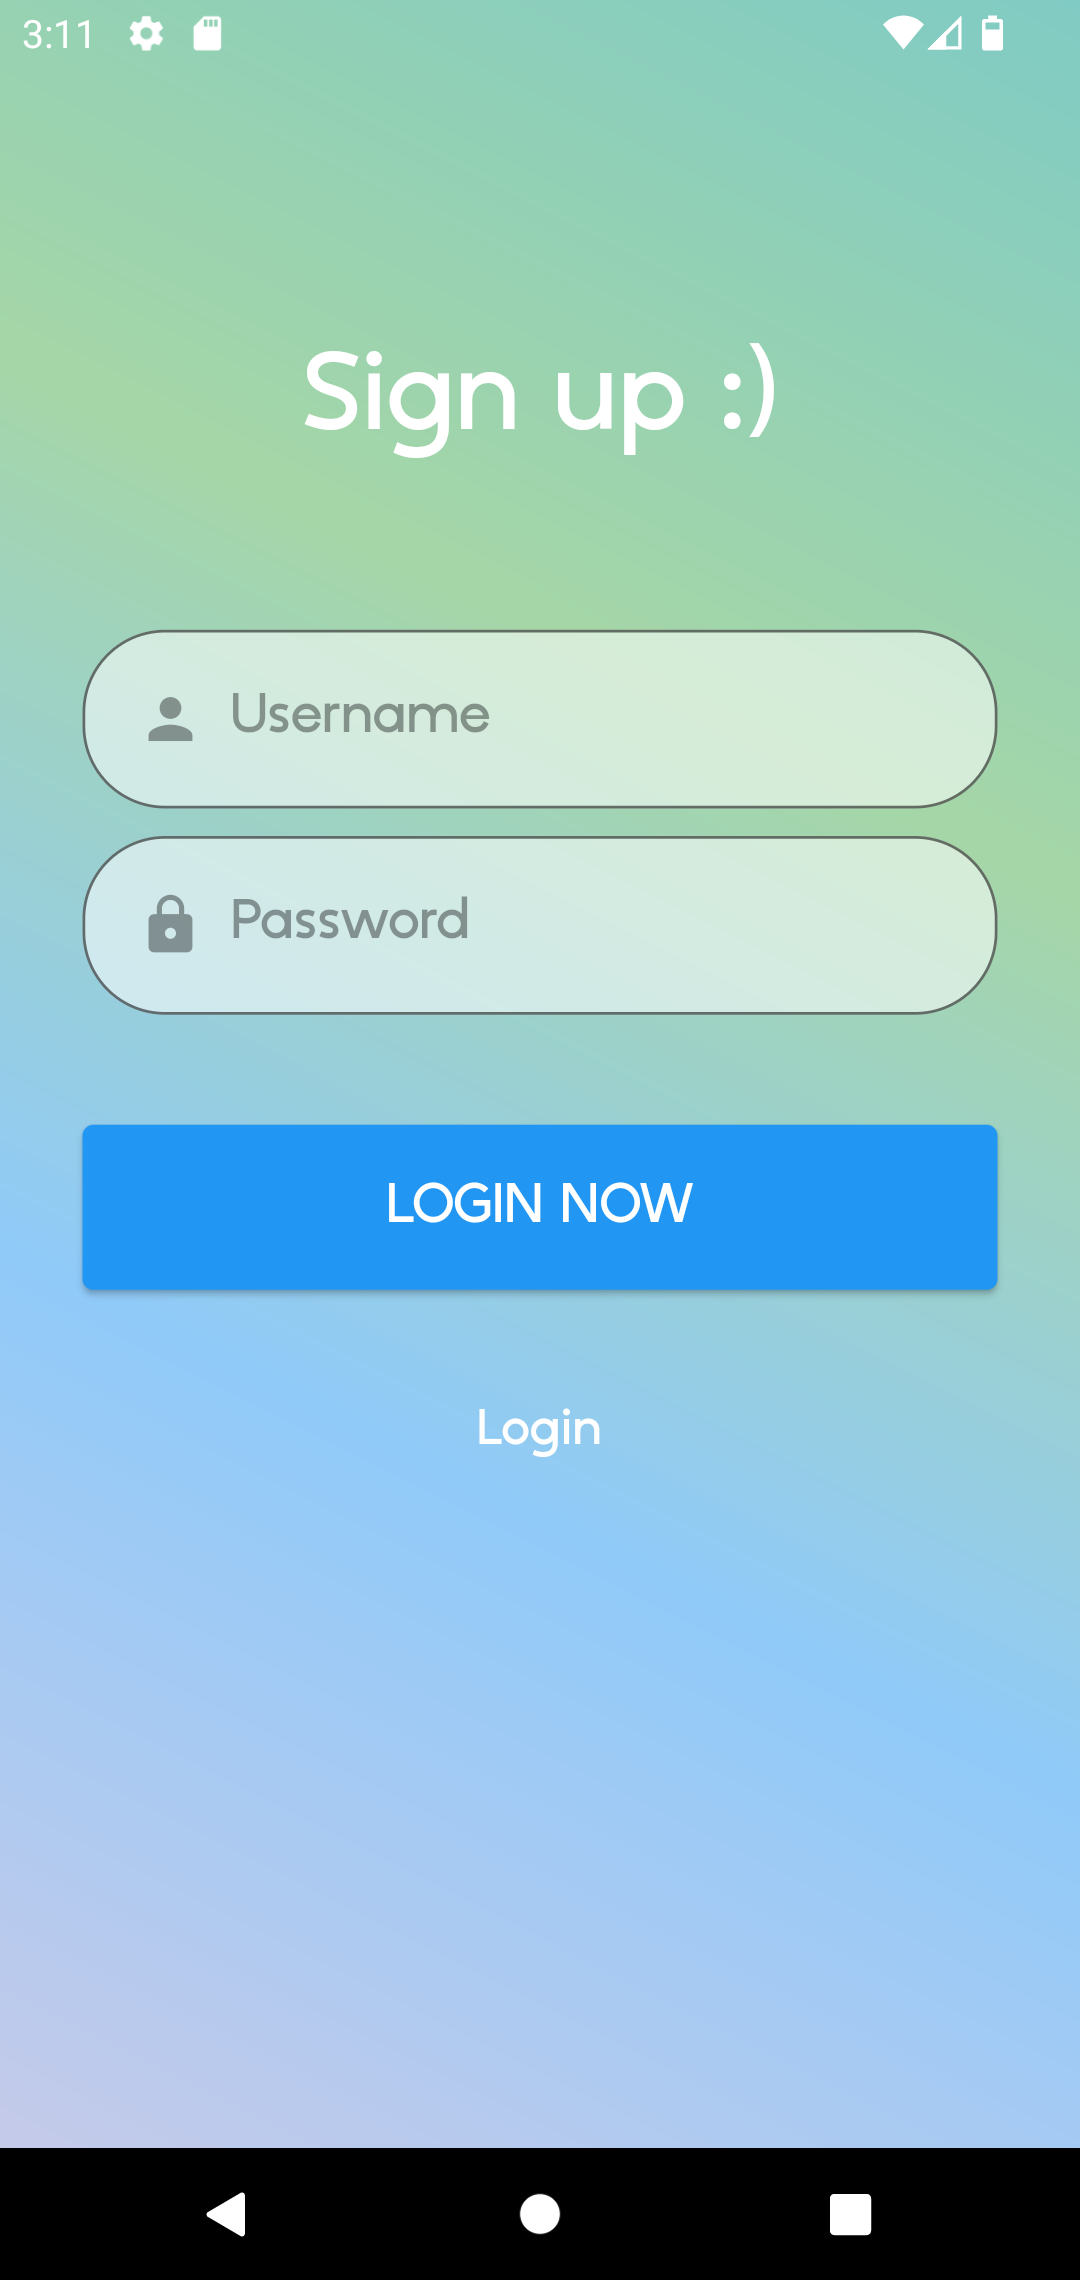
\includegraphics[width=0.3\textwidth]{Gartner/assets/ss_MAFlussdiagramm_registrierfenster.png}
	\caption{Registrierfenster des GUI}
	\label{fig:MA_Registrierfenster}
\end{figure}

Der erste Bildschirm ist wie in Abbildung \ref{fig:MA_Flussdiagramm} zu erkennen entweder das Loginfenster oder der Homescreen mit der Datenansicht. Falls man die App zum ersten Mal �ffnet oder sich in der letzten Session abgemeldet hat, ist das in Abbildung \ref{fig:MA_Loginfenster} zu sehende Loginfenster der Startpunkt. Von hier aus kann sich der Benutzer entweder einloggen, wenn er schon einen Account hat, oder zum Registrierfenster, wie in Abbildung \ref{fig:MA_Registrierfenster} gezeigt, wechseln, um sich zu registrieren. Wenn die Registrierung erfolgreich war, wird wieder zum Loginfenster geleitet. Es gibt aber auch die M�glichkeit, ohne Registrierung wieder zum Loginfenster zu wechseln. In beiden F�llen muss der Login im Loginfenster erfolgen, um die Datenansicht zu laden. \\

\begin{figure}[H]
	\centering
		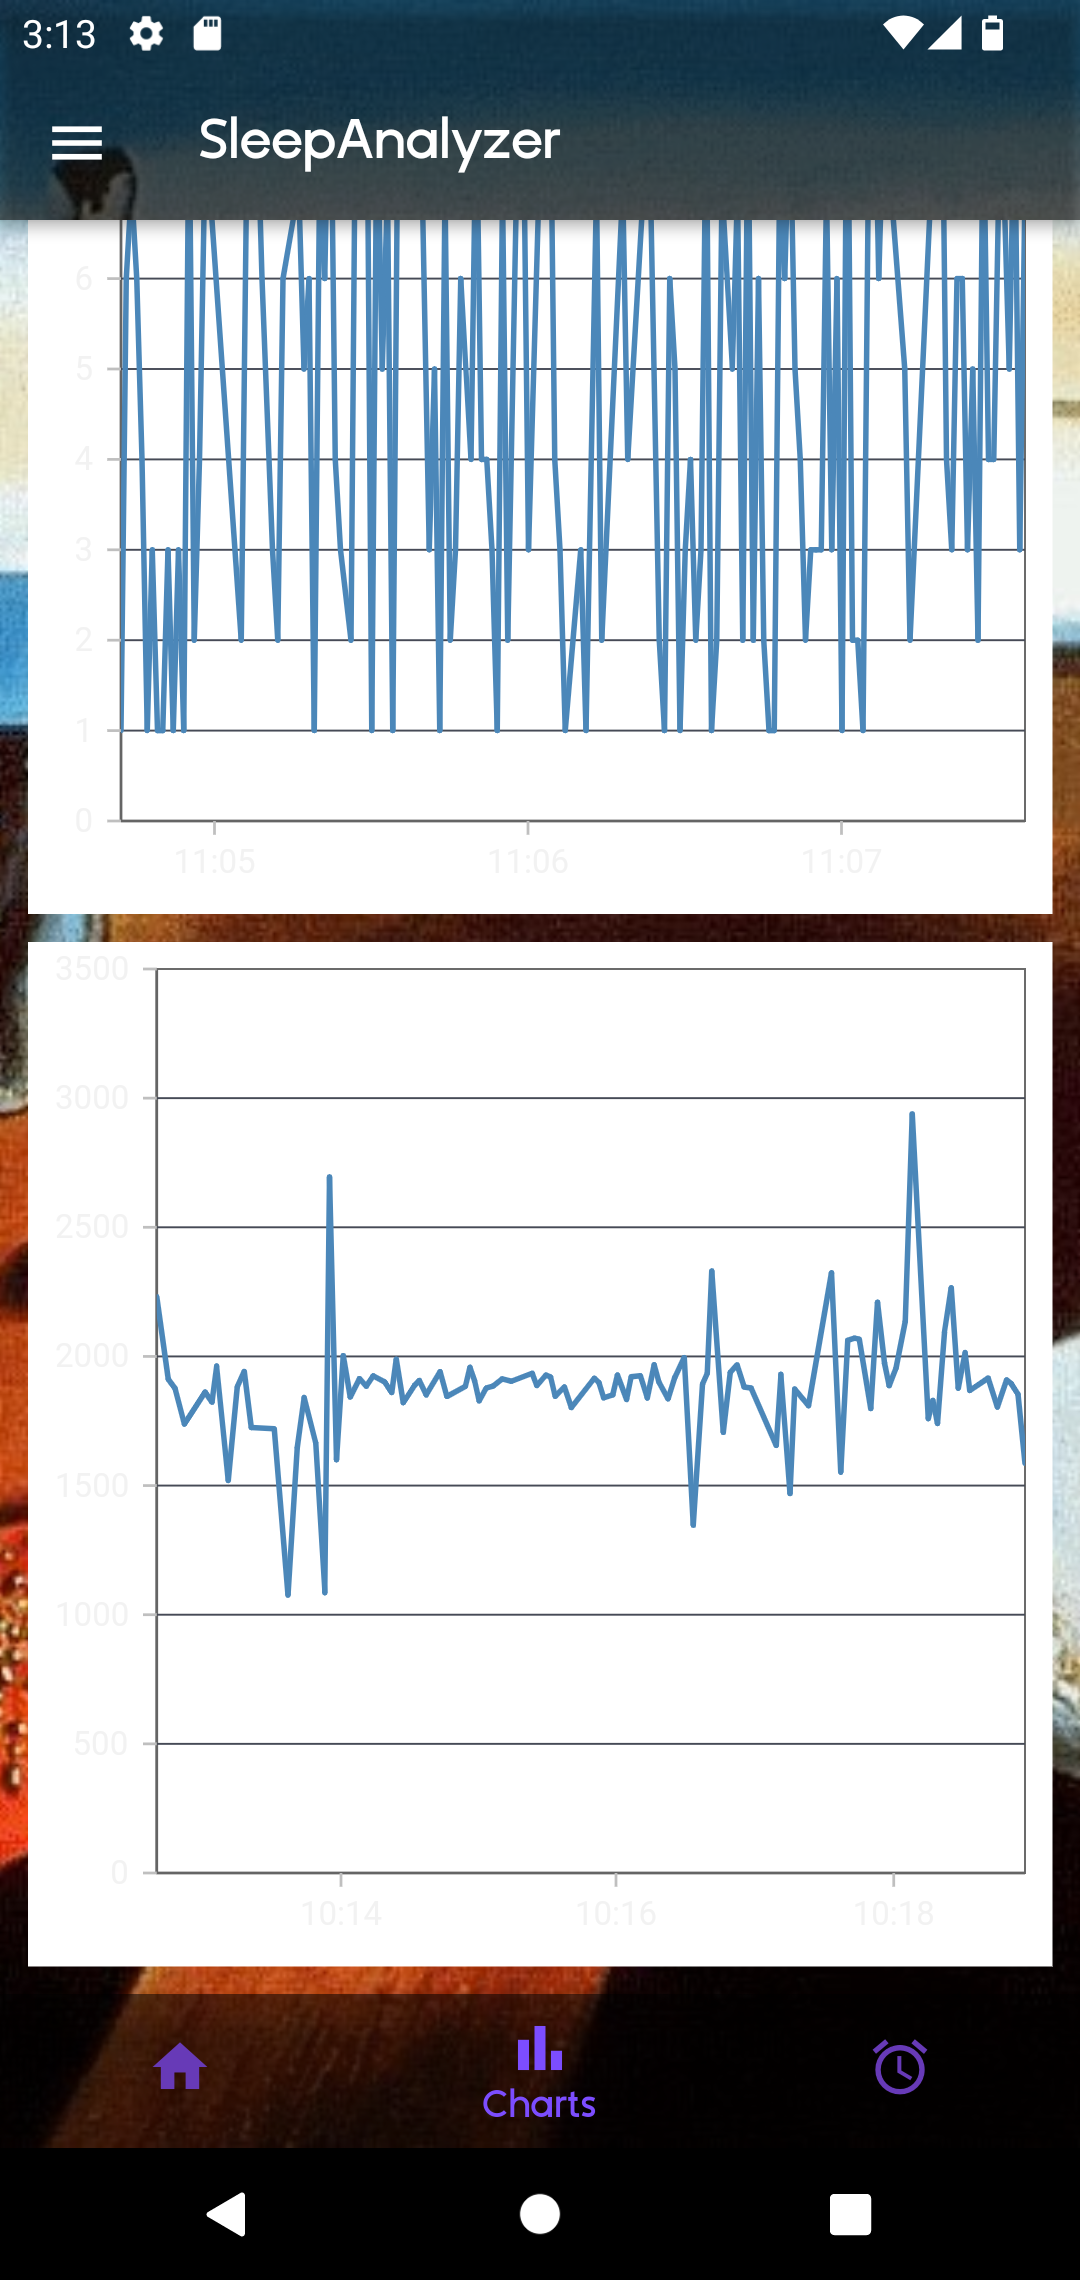
\includegraphics[width=0.3\textwidth]{Gartner/assets/ss_MAFlussdiagramm_datenansicht.png}
	\caption{Datenansicht des GUI}
	\label{fig:MA_Datenansicht}
\end{figure}

Im Fall, dass der User sich bereits einmal eingeloggt und in der letzten Session nicht abgemeldet hat, wird direkt die Datenansicht geladen. Hier gibt es, wie in Abbildung \ref{fig:MA_Datenansicht} zu sehen, eine Navigationsleiste am unteren Ende des Bildschirms, mit dem ausgew�hlt werden kann, ob die Daten- oder Weckeransicht gezeigt wird. \\
In der Datenansicht werden alle Messergebnisse der EOG-Messungen eines Benutzers angezeigt. Hier gibt es, abgesehen vom Scrollfeature, keine Interaktionsm�glichkeiten. \\

\begin{figure}[H]
	\centering
		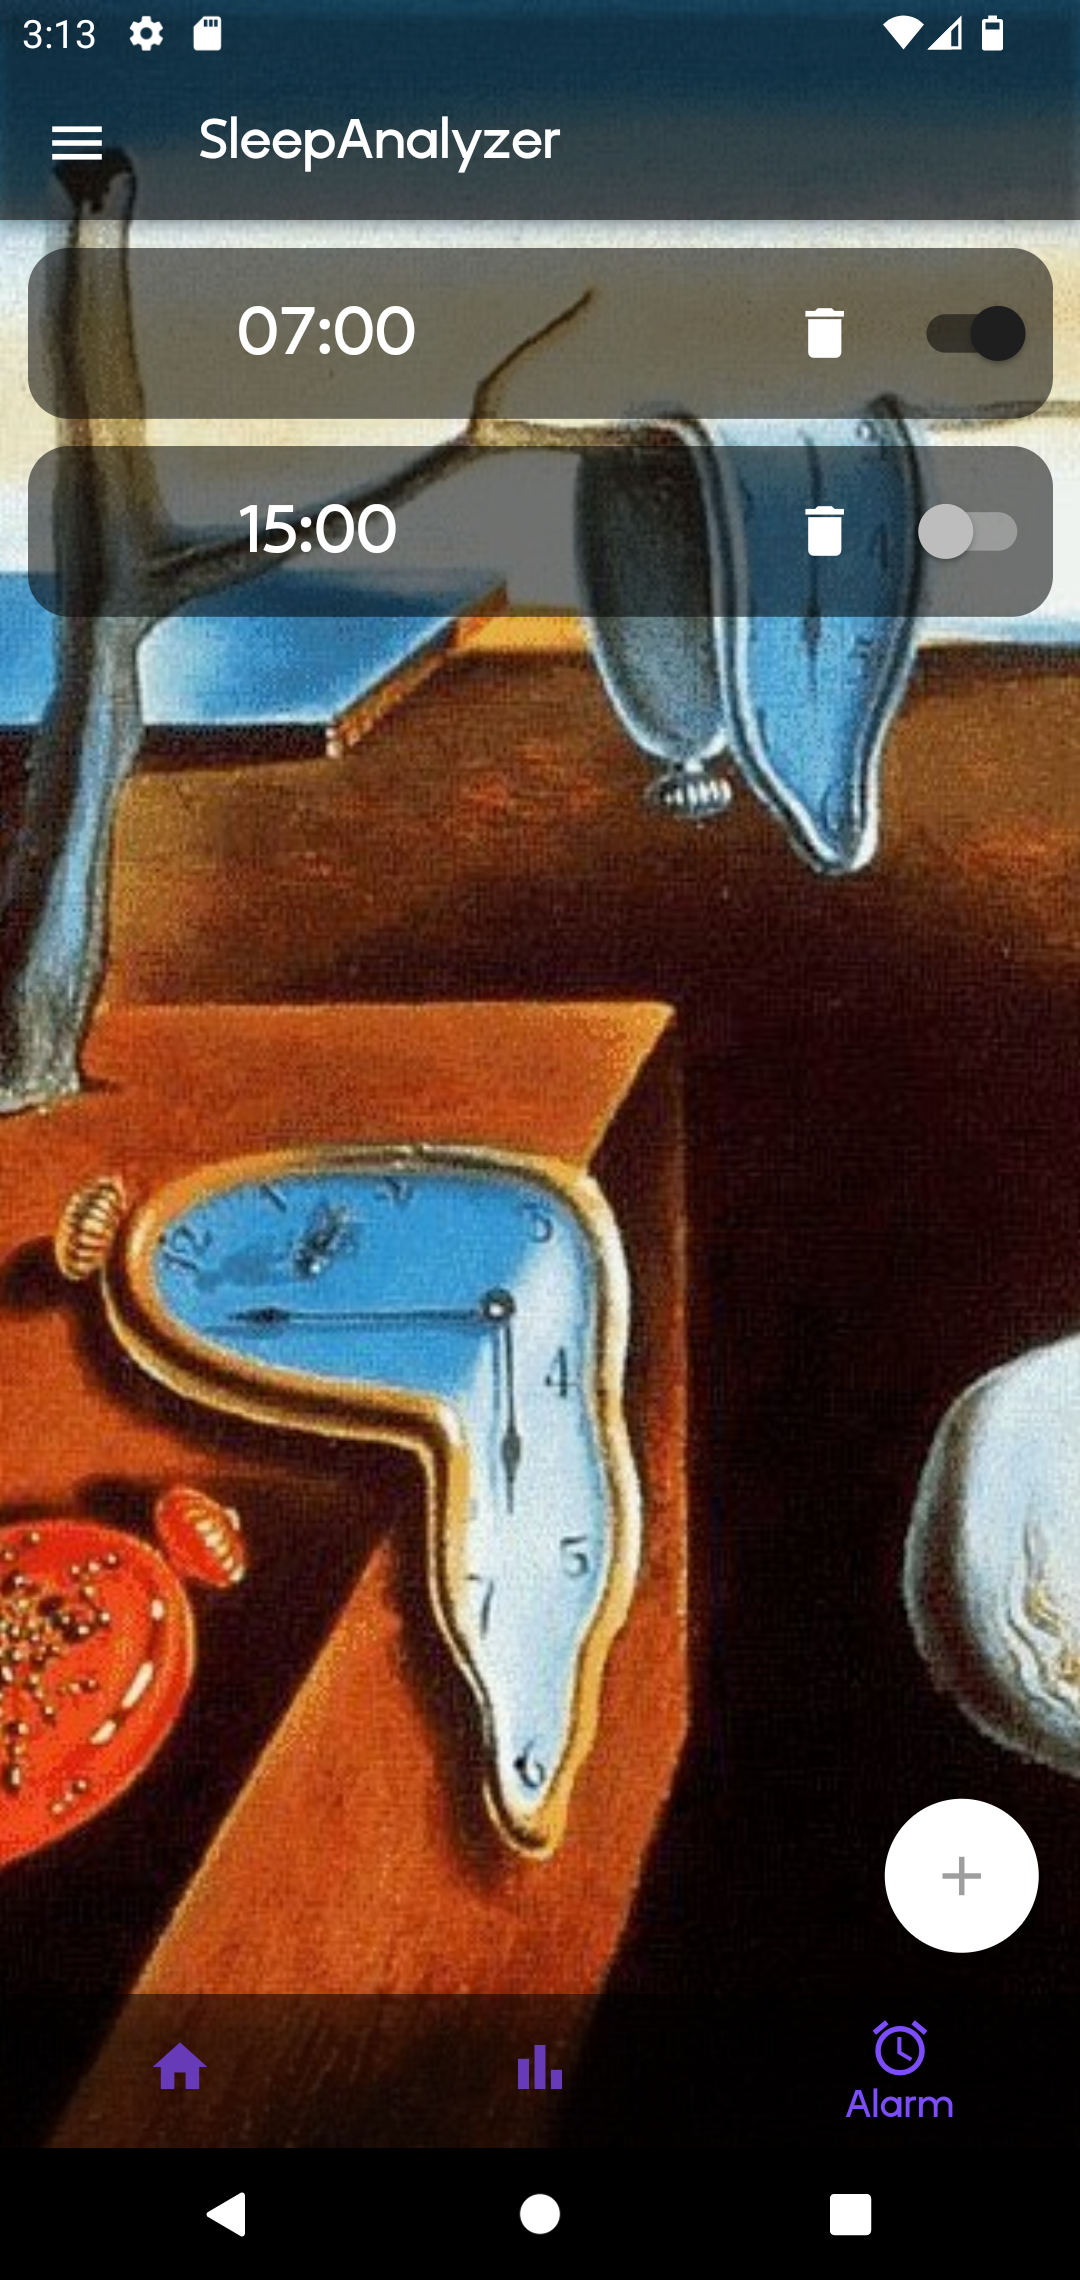
\includegraphics[width=0.3\textwidth]{Gartner/assets/ss_MAFlussdiagramm_weckeransicht.png}
	\caption{Weckeransicht des GUI}
	\label{fig:MA_Weckeransicht}
\end{figure}

Die Weckeransicht, gezeigt in Abbildung \ref{fig:MA_Weckeransicht}, erm�glicht eine Verwaltung der Weckerfunktion. M�gliche Interaktionen hier sind das Hinzuf�gen oder Entfernen und das Ein- oder Ausschalten eines Weckers. Hinzugef�gte Wecker werden ebenfalls hier angezeigt. \\

\begin{figure}[H]
	\centering
		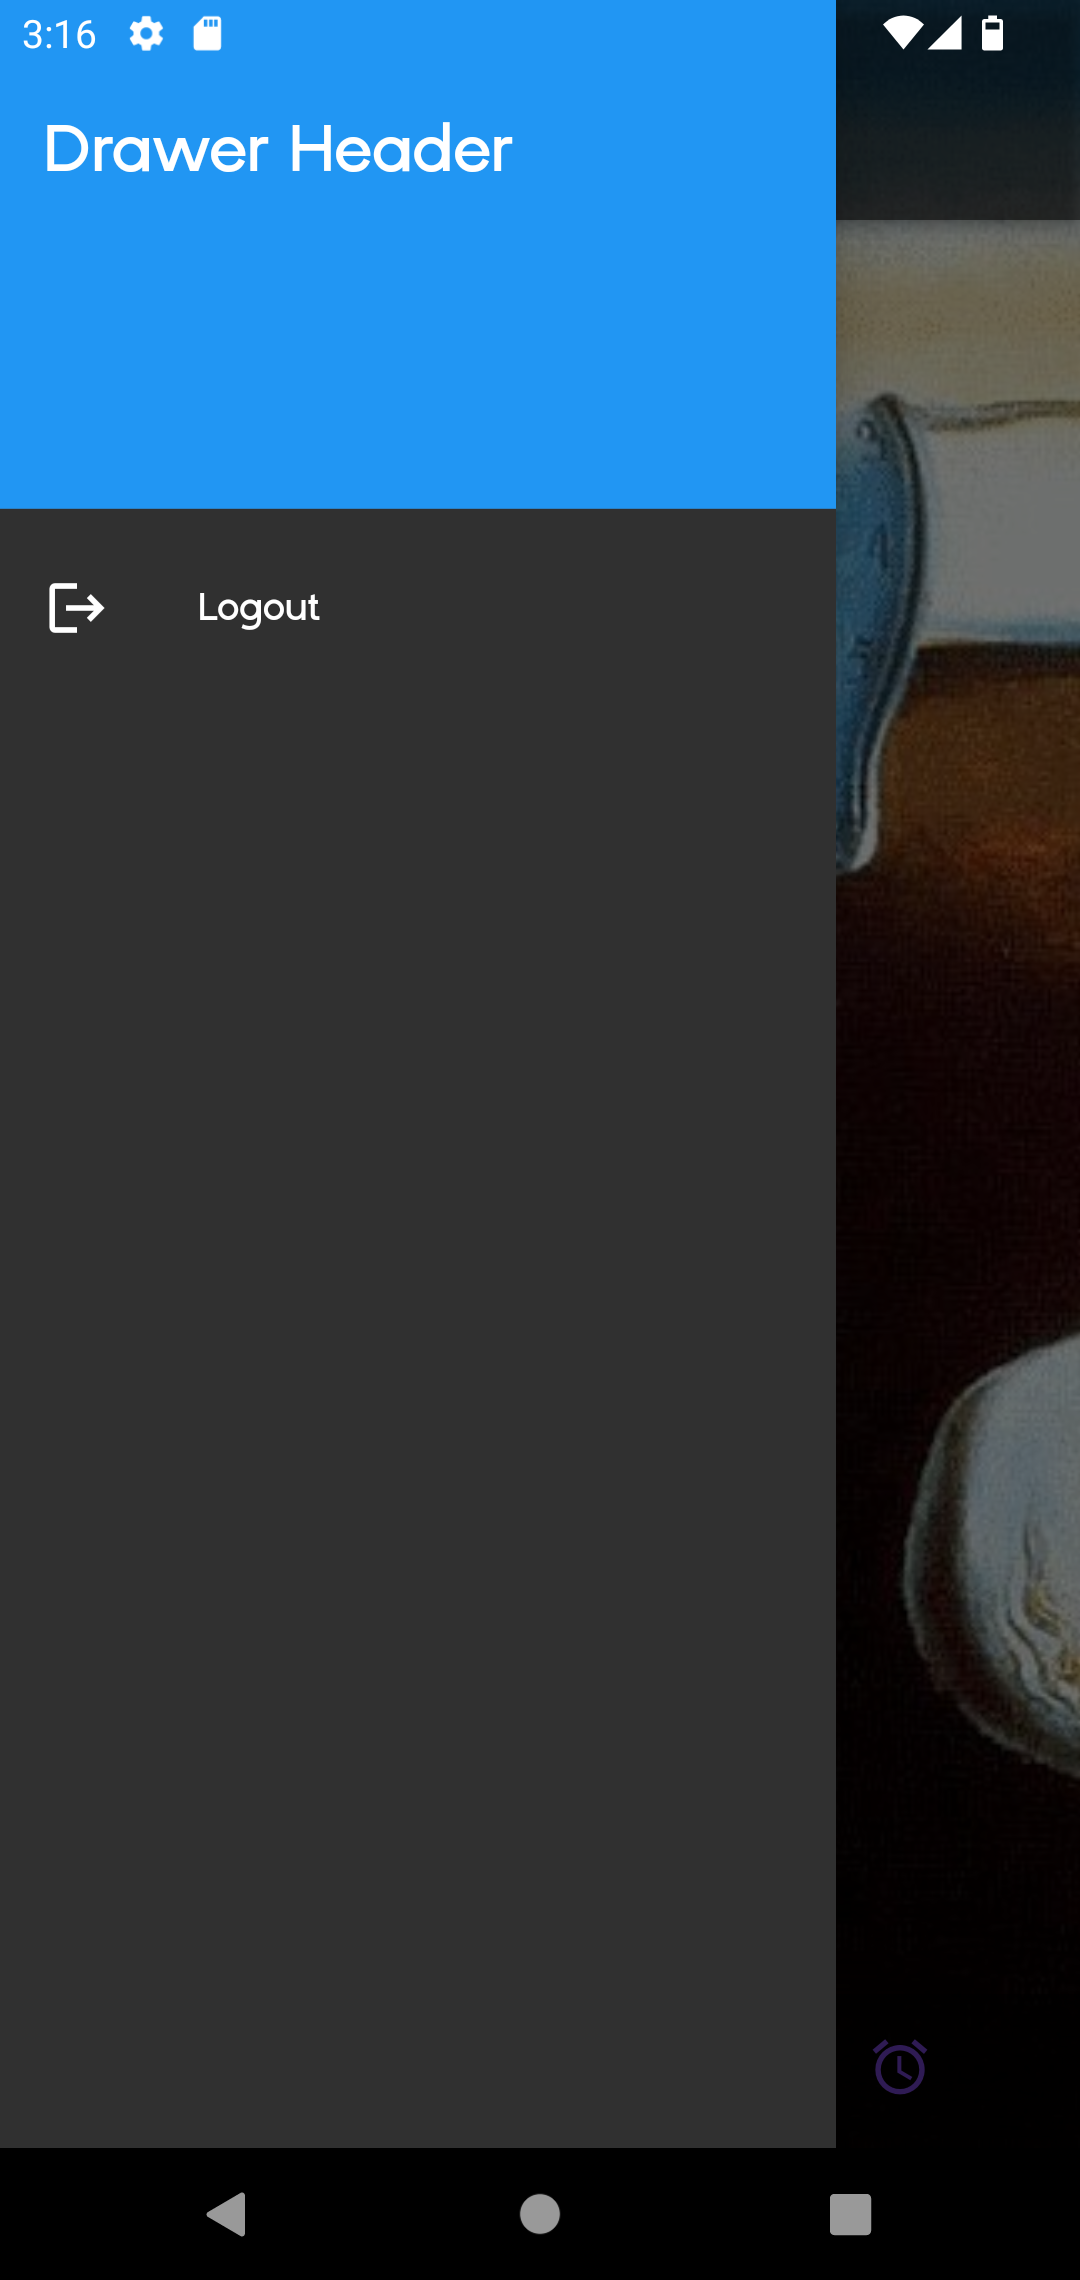
\includegraphics[width=0.3\textwidth]{Gartner/assets/ss_MAFlussdiagramm_logout.png}
	\caption{Logout des GUI}
	\label{fig:MA_Logout}
\end{figure}

Wie bereits in Abbildung \ref{fig:MA_Datenansicht} und \ref{fig:MA_Weckeransicht} zu erkennen, ist links oben in der Ansicht ein Menu Button implementiert. Das dahinterliegende Menu mit der Logout-Funktion ist in Abbildung \ref{fig:MA_Logout} zu sehen. 